\exercisesheader{}

% 19 - course_satisfaction_sections

\eoce{\qt{Course satisfaction across sections\label{course_satisfaction_sections}} 
A large college class has 160 students. All 160 students attend the lectures 
together, but the students are divided into 4 groups, each of 40 students, 
for lab sections administered by different teaching assistants. The professor 
wants to conduct a survey about how satisfied the students are with the course, 
and he believes that the lab section a student is in might affect the student's 
overall satisfaction with the course.
\begin{parts}
\item What type of study is this?
\item Suggest a sampling strategy for carrying out this study.
\end{parts}
}{}

% 20 - housing_proposal_dorms

\eoce{\qt{Housing proposal across dorms\label{housing_proposal_dorms}} On a large 
college campus first-year students and sophomores live in dorms located on 
the eastern part of the campus and juniors and seniors live in dorms located 
on the western part of the campus. Suppose you want to collect student opinions 
on a new housing structure the college administration is proposing and you want 
to make sure your survey equally represents opinions from students from all years.
\begin{parts}
\item What type of study is this?
\item Suggest a sampling strategy for carrying out this study.
\end{parts}
}{}

% 21 - internet_life_expectancy

\eoce{\qt{Internet use and life expectancy\label{internet_life_expectancy}} The 
following scatterplot was created as part of a study evaluating the 
relationship between estimated life expectancy at birth (as of 2014) and 
percentage of internet users (as of 2009) in 208 countries for which such 
data were available.\footfullcite{data:ciaFactbook}

\noindent\begin{minipage}[c]{0.44\textwidth}
\begin{parts}
\item Describe the relationship between life expectancy and percentage of 
internet users.
\item What type of study is this?
\item State a possible confounding variable that might explain this relationship 
and describe its potential effect.
\end{parts} \vspace{15mm}
\end{minipage}
\begin{minipage}[r]{0.55\textwidth}
\tabspecial{tableau-scatter-lifeexp-internetusers}{
\hfill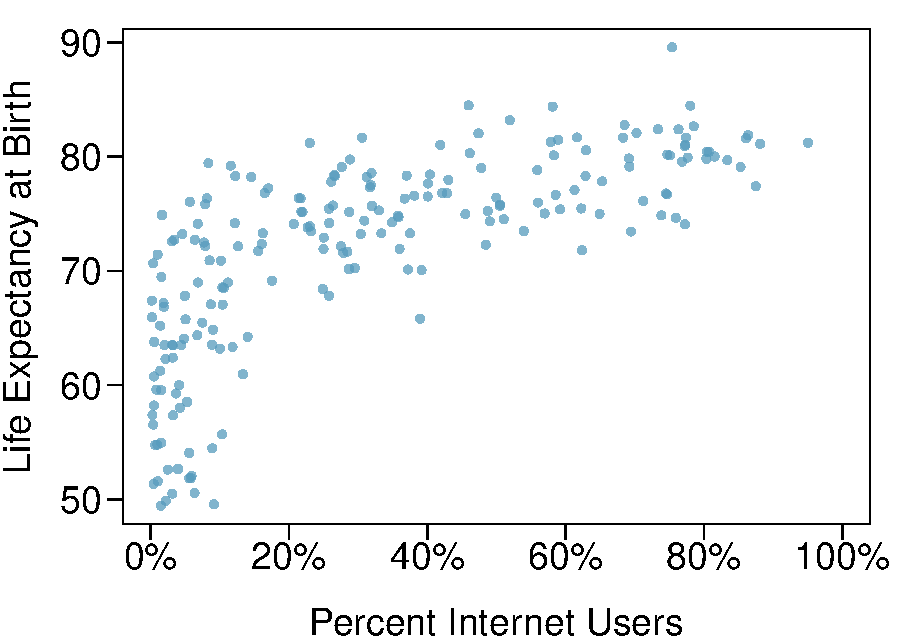
\includegraphics[width = 0.87\textwidth]{ch_data_collection/figures/eoce/internet_life_expectancy/internet_life_expectancy}}
\end{minipage}
}{}

% 22 - stressed_out_observational

\eoce{\qt{Stressed out, Part I\label{stressed_out_observational}} A study that 
surveyed a random sample of otherwise healthy high school students found that 
they are more likely to get muscle cramps when they are stressed. The study 
also noted that students drink more coffee and sleep less when they are 
stressed.
\begin{parts}
\item What type of study is this?
\item Can this study be used to conclude a causal relationship between 
increased stress and muscle cramps?
\item State possible confounding variables that might explain the observed 
relationship between increased stress and muscle cramps. 
\end{parts}
}{}

% 23 - evaluate_sampling_methods

\eoce{\qt{Evaluate sampling methods\label{evaluate_sampling_methods}} A university wants to 
determine what fraction of its undergraduate student body support a new \$25 annual fee 
to improve the student union. For each proposed method below, indicate whether 
the method is reasonable or not.
\begin{parts}
\item Survey a simple random sample of 500 students.
\item Stratify students by their field of study, then sample 10\% of students from  
each stratum.
\item Cluster students by their ages (e.g. 18 years old in one cluster, 19 years 
old in one cluster, etc.), then randomly sample three clusters and survey all 
students in those clusters.
\end{parts}
}{}

% 24 - random_digit_dialing

\eoce{\qt{Random digit dialing\label{random_digit_dialing}} The Gallup Poll uses a 
procedure called random digit dialing, which creates phone numbers based on 
a list of all area codes in America in conjunction with the associated number 
of residential households in each area code. Give a possible reason the Gallup 
Poll chooses to use random digit dialing instead of picking phone numbers 
from the phone book.
}{}

% 25 - scope_haters

\eoce{\qt{Haters are gonna hate, study confirms\label{scope_haters}}
A study published in the
\textit{Journal of Personality and Social Psychology}
asked a group of 200 randomly sampled men and
women to evaluate how they felt about various subjects,
such as camping, health care, architecture, taxidermy, 
crossword puzzles, and Japan in order to measure their
attitude towards mostly independent stimuli.
Then, they presented the participants with information
about a new product: a microwave oven. This microwave oven
does not exist, but the participants didn't know this,
and were given three positive and three negative fake reviews.
People who reacted positively to the subjects on the
dispositional attitude measurement also tended to react 
positively to the microwave oven, and those who reacted
negatively tended to react negatively to it.
Researchers concluded that ``some people tend to 
like things, whereas others tend to dislike things, and a more thorough 
understanding of this tendency will lead to a more thorough understanding of 
the psychology of attitudes." \footfullcite{Hepler:2013}
\begin{parts}
\item What are the cases?
\item What is (are) the response variable(s) in this study?
\item What is (are) the explanatory variable(s) in this study?
\item Does the study employ random sampling?
\item Is this an observational study or an experiment? Explain your reasoning.
\item Can we establish a causal link between the explanatory and response 
variables?
\item Can the results of the study be generalized to the population at large?
\end{parts}
}{}

% 26 - family_size_bias

\eoce{\qt{Family size\label{family_size}} Suppose we want to estimate household 
size, where a ``household" is defined as people living together in the 
same dwelling, and sharing living accommodations. If we select students 
at random at an elementary school and ask them what their family size is, 
will this be a good measure of household size? Or will our average be 
biased? If so, will it overestimate or underestimate the true value?
}{}

% 27 - sampling_strategies

\eoce{\qt{Sampling strategies\label{sampling_strategies}} A statistics student who is curious about the relationship between the amount of time students spend on social networking sites and their performance at school decides to conduct a survey. Various research strategies for collecting data are described below. In each, name the sampling method proposed and any bias you might expect.
\begin{parts}
\item He randomly samples 40 students from the study's population, gives them the survey, asks them to fill it out and bring it back the next day.
\item He gives out the survey only to his friends, making sure each one of them fills out the survey.
\item He posts a link to an online survey on Facebook and asks his friends to fill out the survey.
\item He randomly samples 5 classes and asks a random sample of students from those classes to fill out the survey.
\end{parts}
}{}

% 28 - reading_paper

\eoce{\qt{Reading the paper\label{reading_paper}} Below are excerpts from two 
articles published in the \emph{NY Times}:
\begin{parts}
\item An article titled \emph{Risks: Smokers Found More Prone to Dementia} 
states the following: \footfullcite{news:smokingDementia}
\begin{adjustwidth}{1em}{1em}
{\footnotesize ``Researchers analyzed data from 23,123 health plan members who 
participated in a voluntary exam and health behavior survey from 1978 to 1985, 
when they were 50-60 years old. 23 years later, about 25\% of the group had 
dementia, including 1,136 with Alzheimer's disease and 416 with vascular 
dementia. After adjusting for other factors, the researchers concluded that 
pack-a-day smokers were 37\% more likely than nonsmokers to develop dementia, 
and the risks went up with increased smoking; 44\% for one to two packs a day; 
and twice the risk for more than two packs."}
\end{adjustwidth}
Based on this study, can we conclude that smoking causes dementia later in 
life? Explain your reasoning.
\item Another article titled \emph{The School Bully Is Sleepy} states the 
following: \footfullcite{news:bullySleep}
\begin{adjustwidth}{1em}{1em}
{\footnotesize ``The University of Michigan study, collected survey data from 
parents on each child's sleep habits and asked both parents and teachers to 
assess behavioral concerns. About a third of the students studied were 
identified by parents or teachers as having problems with disruptive behavior 
or bullying. The researchers found that children who had behavioral issues and 
those who were identified as bullies were twice as likely to have shown 
symptoms of sleep disorders."}
\end{adjustwidth}
A friend of yours who read the article says, ``The study shows that sleep 
disorders lead to bullying in school children." Is this statement justified? 
If not, how best can you describe the conclusion that can be drawn from this 
study?
\end{parts}
}{}
